\subsection{(Domain)model}
\textbf{Structure} \\\\
The system includes three different kind of entities:
\begin{itemize}
	\item \textbf{Robot}: reactive and atomic entity - Receives commands from the user interface, can emit and sense events and can send messages;
	\item \textbf{Sonar}: proactive and atomic entity - Emits the distances values to the radar entity;
	\item \textbf{Radar}: reactive, proactive and composed entity - Composed by 2 graphical interfaces, the first used to display sonar's distance values and the second to display user's command.
\end{itemize}
\textbf{Interaction} \\\\
Interactions can be synchronous or asynchronous and relate to data or data streams. In this second case they may also be isochronous. 
\begin{itemize}
	\item \textbf{Asynchronous interaction:} communication is "buffered" without limitation on buffer size. The emitter should not expect any return information even when it sends information to a specific recipient. Receiver only waits when the buffer is empty. In the case of stream, there are no time constraints for reception.
	\item \textbf{Synchronous interaction:} communication takes place without the use of any buffer. The issuer and the desinerium exchange information by unifying their activities conceptually. In the case of streams, the recipient expects to receive the data with a delay that does not exceed a predetermined maximum.
	\item \textbf{Isochronous interaction:} affects only streams; the recipient expects to receive the data with a delay between a minimum and a maximum.
\end{itemize}
Requirements show the system's distributed and heterogeneous nature reason that no assumptions were made regarding the technology of the nodes. After several talks with the costumer, the following specifications also emerged: 
\begin{itemize}
	\item Sonar's distance values is an asynchronous interaction between sonar and radar;
	\item Alarm is an asynchronous communication send from the radar to the robot;
	\item The photo taken by the robot must be sent to the console with an asynchronous communication point to point;
	\item User command is an asynchronous communication send from console to the robot;
	\item Radar notify to the robot when it reaches a sonar with an asynchronous interaction.
\end{itemize}
The interaction between the entities that compose the system can be formalized by a sequence diagram.
\begin{figure}[h]
	\centering
	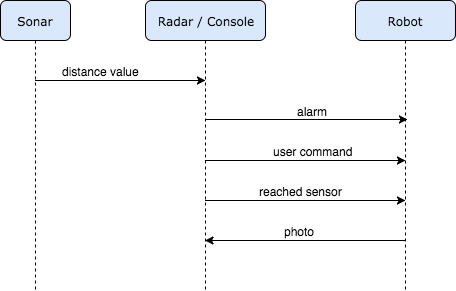
\includegraphics[width=\linewidth]{Interaction-Domain-Model.png}
	\caption{Interactions between the entities}
\end{figure}
\\\textbf{Behaviour} \\\\
The behaviour of the entities can be modelled through simple finite state machine diagrams.
\\\\
\textbf{Sonar}
\begin{figure}[h]
	\centering
	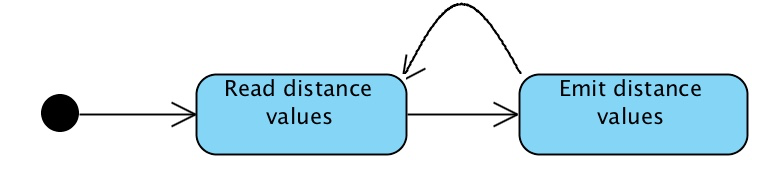
\includegraphics[width=\linewidth]{sonar.png}
	\caption{FSM for Sonar}
\end{figure}
\clearpage
\textbf{Console}
\begin{figure}[h]
	\centering
	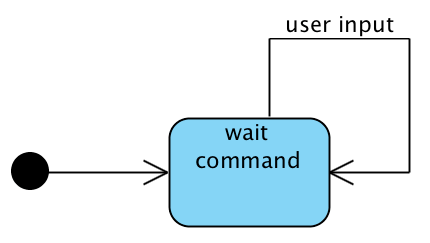
\includegraphics[width=7cm]{Console.png}
	\caption{FSM for Console}
\end{figure}
\\\\
\textbf{Radar}
\begin{figure}[h]
	\centering
	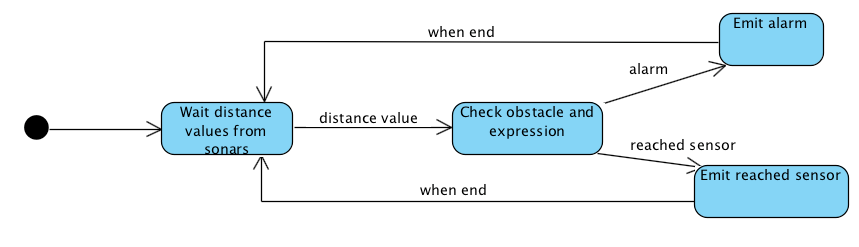
\includegraphics[width=\linewidth]{radar.png}
	\caption{FSM for Radar}
\end{figure}
\clearpage
\textbf{Robot}
\begin{figure}[h]
	\centering
	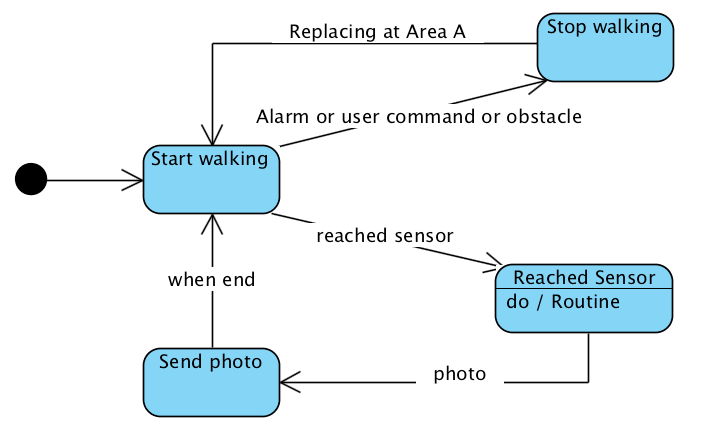
\includegraphics[width=\linewidth]{robot.png}
	\caption{FSM for Robot}
\end{figure}